\documentclass[aspectratio=169]{beamer}
\usepackage[utf8]{inputenc}
\usepackage[T1]{fontenc}
\usepackage{lmodern}
\usepackage{xcolor}
\usepackage[portuguese]{babel}

\definecolor{BgCream}{HTML}{FAF8F5}
\definecolor{TextEspresso}{HTML}{4A4238}
\definecolor{NudeTaupe}{HTML}{BFAFA6}
\definecolor{SoftBlush}{HTML}{D9C5B2}

\setbeamertemplate{navigation symbols}{}
\setbeamercolor{background canvas}{bg=BgCream}
\setbeamercolor{normal text}{fg=TextEspresso}
\setbeamercolor{structure}{fg=TextEspresso}

\setbeamertemplate{itemize item}{\color{NudeTaupe}\textendash}
\setbeamertemplate{itemize subitem}{\color{NudeTaupe}\(\circ\)}

\setbeamerfont{title}{size=\huge, series=\bfseries}
\setbeamerfont{frametitle}{size=\Large, series=\bfseries}

\setbeamertemplate{title page}{
  \vspace*{1.5cm}
  \begin{center}
    \usebeamerfont{title}\textcolor{TextEspresso}{\inserttitle}\par
    \vspace{0.35cm}
    {\large\textcolor{NudeTaupe}{\insertsubtitle}}\par
    \vspace{0.6cm}
    {\color{NudeTaupe}\rule{2.5cm}{0.5pt}}\par
    \vspace{0.8cm}
    \usebeamerfont{author}\textcolor{TextEspresso}{\insertauthor}\par
    \vspace{0.3cm}
    \usebeamerfont{institute}\small\textcolor{NudeTaupe}{\insertinstitute \quad|\quad \insertdate}
  \end{center}
}

\setbeamertemplate{frametitle}{
  \vspace*{0.8cm}
  \usebeamerfont{frametitle}\insertframetitle\par
  \vspace*{-0.1cm}
  {\color{NudeTaupe}\rule{1.5cm}{0.5pt}}
  \vspace*{0.2cm}
}

\newenvironment{ideiachave}{
  \vspace{0.5cm}
  \begin{center}
  \color{TextEspresso}
  \itshape\Large
}{
  \end{center}
  \vspace{0.5cm}
}

\usepackage{csquotes}

\title{Virtualização de Sistemas}
\subtitle{Infraestruturas de Computação na Nuvem, Aula 03}
\author{Catarina Silva}
\institute{ESTGA, Universidade de Aveiro}
\date{2026}

\begin{document}

\begin{frame}[plain]
  \titlepage
\end{frame}

\begin{frame}
\frametitle{Agenda \textcolor{NudeTaupe}{\small(1/2)}}
\begin{itemize}
    \setlength\itemsep{0.4cm}
    \item Conceito de virtualização e motivação.
    \item Os requisitos de Popek e Goldberg.
    \item Hypervisors tipo 1 vs tipo 2.
    \item Estratégias de virtualização de CPU.
    \item Os anéis de privilégio e o problema do x86.
    \item Trap-and-emulate: como o hypervisor intervém.
\end{itemize}
\end{frame}

\begin{frame}
\frametitle{Agenda \textcolor{NudeTaupe}{\small(2/2)}}
\begin{itemize}
    \setlength\itemsep{0.4cm}
    \item Virtualização de memória, rede e armazenamento.
    \item Memory overcommit: KSM e ballooning.
    \item Virtualização de I/O: emulação, passthrough e SR-IOV.
    \item Formatos de disco virtual e thin provisioning.
    \item Snapshots e clones.
    \item Migração ao vivo e overhead de virtualização.
    \item KVM, LXC e a plataforma Proxmox VE.
\end{itemize}
\end{frame}

\begin{frame}
\frametitle{Conceito de Virtualização e Motivação}
\begin{itemize}
    \setlength\itemsep{0.4cm}
    \item Virtualização: criação de uma versão abstrata (virtual) de um recurso físico, permitindo executar múltiplos sistemas isolados sobre o mesmo hardware.
    \item \textbf{Consolidação:} redução do número de máquinas físicas necessárias, melhorando o aproveitamento de recursos.
    \item \textbf{Isolamento:} falhas ou comprometimentos numa VM não afetam diretamente as restantes.
    \item \textbf{Portabilidade:} uma VM pode ser movida, copiada ou replicada independentemente do hardware subjacente.
\end{itemize}
\end{frame}

\begin{frame}
\frametitle{Os Requisitos de Popek e Goldberg}
\begin{itemize}
    \setlength\itemsep{0.4cm}
    \item Em 1974, Popek e Goldberg formalizaram três propriedades que um hypervisor deve garantir.
    \item \textbf{Equivalência}: um programa a correr na VM comporta-se como correria diretamente no hardware.
    \item \textbf{Controlo de recursos}: o hypervisor mantém controlo total sobre os recursos físicos atribuídos.
    \item \textbf{Eficiência}: a maioria das instruções executa diretamente no processador, sem intervenção do hypervisor.
    \item Estes critérios continuam a ser a referência para avaliar qualquer solução de virtualização.
\end{itemize}
\end{frame}

\begin{frame}
\frametitle{Hypervisors Tipo 1 vs Tipo 2}
\begin{itemize}
    \setlength\itemsep{0.4cm}
    \item \textbf{Tipo 1 (bare-metal):} executa diretamente sobre o hardware, sem sistema operativo intermédio. Exemplos: VMware ESXi, KVM, Xen, Hyper-V.
    \item \textbf{Tipo 2 (hosted):} executa como uma aplicação sobre um sistema operativo anfitrião. Exemplos: VirtualBox, VMware Workstation.
    \item Hypervisors tipo 1 têm menor overhead e são a escolha habitual em datacenters de produção.
    \item Hypervisors tipo 2 são mais simples de instalar e adequados a ambientes de desenvolvimento e teste.
\end{itemize}
\end{frame}

\begin{frame}
\frametitle{As Duas Arquiteturas de Hypervisor}
\vfill
\begin{center}
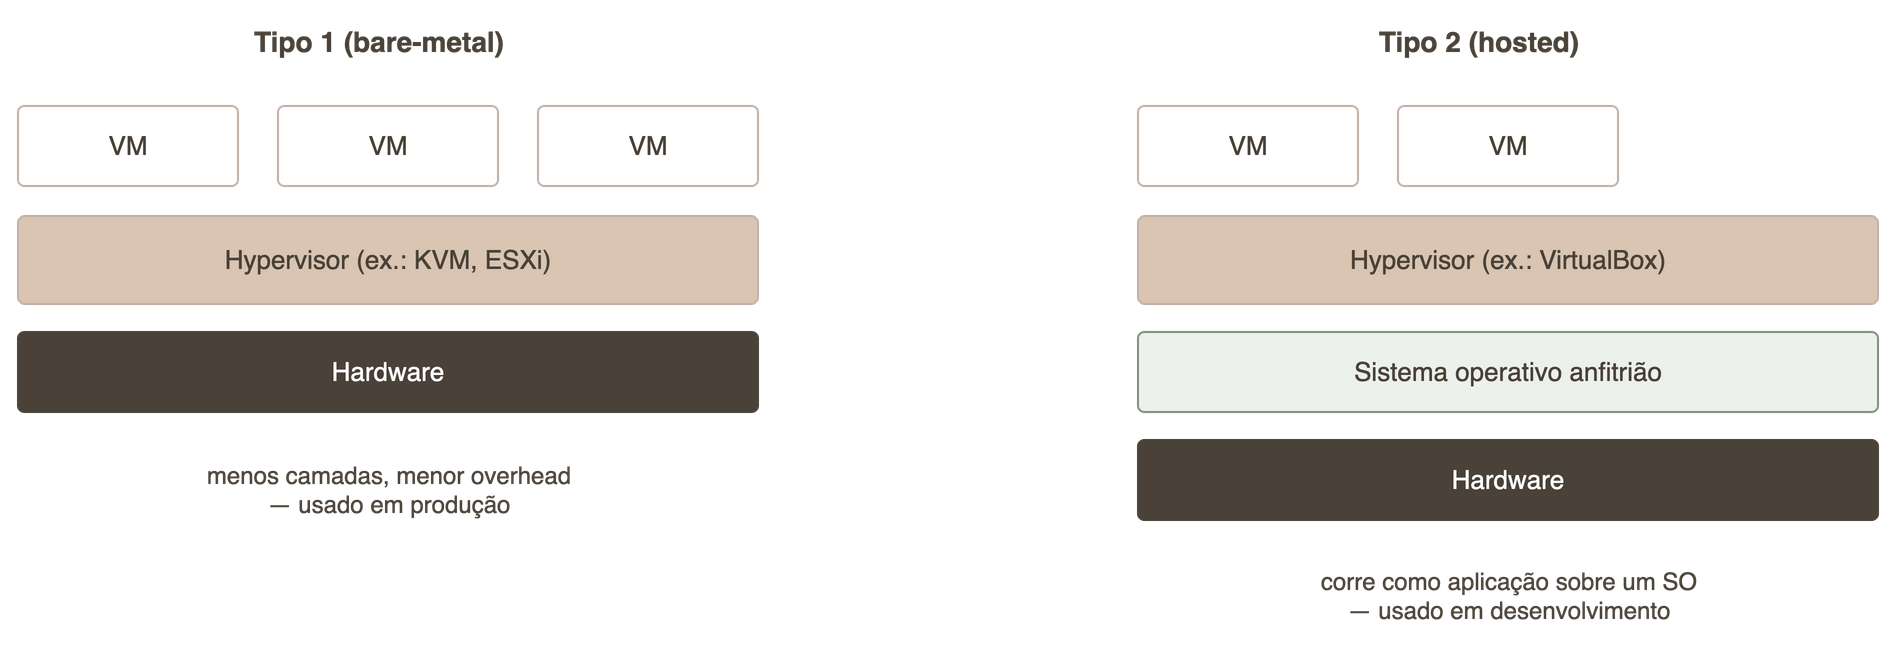
\includegraphics[width=0.97\textwidth,height=0.70\textheight,keepaspectratio]{../Diagramas/a03-hypervisors.png}
\end{center}
\vfill
\end{frame}


\begin{frame}
\frametitle{Estratégias de Virtualização de CPU}
\begin{itemize}
    \setlength\itemsep{0.4cm}
    \item \textbf{Virtualização completa:} o hypervisor emula totalmente o hardware; o sistema convidado corre sem modificações.
    \item \textbf{Paravirtualização:} o sistema convidado é adaptado para comunicar diretamente com o hypervisor, reduzindo overhead.
    \item \textbf{Virtualização assistida por hardware:} extensões de processador (Intel VT-x, AMD-V) que aceleram a execução de instruções privilegiadas.
    \item A maioria dos hypervisors modernos combina virtualização completa com suporte de hardware.
\end{itemize}
\end{frame}

\begin{frame}
\frametitle{Anéis de Privilégio e o Problema do x86}
\begin{itemize}
    \setlength\itemsep{0.4cm}
    \item A arquitetura x86 define \textbf{anéis de privilégio}, do anel 0 (máximo privilégio, kernel) ao anel 3 (aplicações).
    \item Um sistema operativo convidado espera correr no anel 0, mas numa VM esse lugar pertence ao hypervisor.
    \item Problema histórico: no x86 clássico, certas instruções privilegiadas falhavam silenciosamente em vez de gerarem uma exceção capturável pelo hypervisor.
    \item Soluções: tradução binária dinâmica (reescrever instruções problemáticas em tempo de execução) ou paravirtualização.
    \item \textbf{Intel VT-x} e \textbf{AMD-V} resolveram o problema na raiz, criando um modo de execução dedicado ao hypervisor.
\end{itemize}
\end{frame}

\begin{frame}
\frametitle{Trap-and-Emulate: Como o Hypervisor Intervém}
\begin{itemize}
    \setlength\itemsep{0.4cm}
    \item Popek e Goldberg classificam as instruções em três tipos: \textbf{seguras} (sem impacto global, executam livremente), \textbf{sensíveis} (acedem a hardware ou tabelas de páginas) e \textbf{privilegiadas} (geram uma exceção -- \textit{trap} -- se executadas em modo utilizador).
    \item O código convidado corre como uma aplicação normal; quando emite uma instrução sensível, o processador gera um \textit{trap} e devolve o controlo ao hypervisor.
    \item O hypervisor apanha o \textit{trap}, emula o efeito da instrução (por exemplo, uma escrita em disco vira uma escrita num ficheiro) e devolve o controlo ao convidado, que não nota a interrupção.
    \item Este mecanismo aplica-se a múltiplos subsistemas: CPU e registos, unidade de gestão de memória (tabelas de páginas), controlador de interrupções e temporizadores, e dispositivos periféricos.
\end{itemize}
\end{frame}

\begin{frame}
\frametitle{Virtualização de Memória e Rede \textcolor{NudeTaupe}{\small(1/2)}}
\begin{itemize}
    \setlength\itemsep{0.4cm}
    \item Virtualização de memória: cada VM tem o seu próprio espaço de endereçamento, gerido pelo hypervisor.
    \item \textbf{Shadow page tables:} o hypervisor mantém uma tabela de páginas própria, traduzindo endereços da VM para endereços físicos.
    \item \textbf{EPT} (Extended Page Tables): suporte de hardware que acelera esta tradução, eliminando parte do overhead das shadow page tables.
\end{itemize}
\end{frame}

\begin{frame}
\frametitle{Virtualização de Memória e Rede \textcolor{NudeTaupe}{\small(2/2)}}
\begin{itemize}
    \setlength\itemsep{0.4cm}
    \item Virtualização de rede: um \textbf{vSwitch} (switch virtual) interliga as interfaces de rede virtuais das VMs entre si e com a rede física.
    \item Permite criar redes isoladas, VLANs virtuais e políticas de tráfego sem alterar o cablagem física.
    \item Virtualização de armazenamento: discos virtuais (ficheiros) que abstraem o armazenamento físico subjacente, permitindo snapshots e migração.
\end{itemize}
\end{frame}

\begin{frame}
\frametitle{Memory Overcommit: KSM e Ballooning}
\begin{itemize}
    \setlength\itemsep{0.4cm}
    \item Num servidor partilhado por várias VMs, atribuir a cada uma a memória máxima "no papel" desperdiça RAM real -- a maior parte de um SO fica em cache e buffers raramente usados.
    \item \textbf{KSM} (Kernel Samepage Merging): o hypervisor deteta páginas de memória idênticas entre VMs semelhantes (o mesmo binário, as mesmas bibliotecas) e funde-as numa só página física, com \textit{copy-on-write} caso uma VM a modifique.
    \item \textbf{Ballooning}: um driver dentro do convidado "infla" um balão, reclamando memória que o SO convidado liberta (via \textit{page cache}); o hypervisor reatribui essa memória a outras VMs sem que o convidado perceba que foi retirada.
    \item Ambos os mecanismos permitem \textit{overcommit} de memória com segurança, mas dependem de suporte explícito na plataforma -- no Proxmox, são opções configuráveis por VM.
\end{itemize}
\end{frame}

\begin{frame}
\frametitle{Formatos de Disco Virtual}
\begin{itemize}
    \setlength\itemsep{0.4cm}
    \item \textbf{raw}: imagem sem estrutura adicional; desempenho máximo, mas sem funcionalidades próprias.
    \item \textbf{qcow2} (QEMU Copy On Write 2): formato nativo do QEMU/KVM, com suporte a snapshots internos, compressão e alocação dinâmica.
    \item \textbf{VMDK} (VMware) e \textbf{VHD/VHDX} (Microsoft): formatos equivalentes noutros ecossistemas.
    \item \textbf{Thin provisioning}: o disco ocupa em armazenamento apenas o espaço efetivamente escrito, não o tamanho nominal declarado.
    \item Permite sobrecomprometer armazenamento (\textit{overcommit}), à custa de exigir monitorização atenta do espaço real disponível.
\end{itemize}
\end{frame}

\begin{frame}
\frametitle{Snapshots e Clones}
\begin{itemize}
    \setlength\itemsep{0.4cm}
    \item \textbf{Snapshot}: captura o estado de uma VM num instante (disco e, opcionalmente, memória), permitindo reverter mais tarde.
    \item Funciona tipicamente por \textit{copy-on-write}: apenas os blocos alterados após o snapshot são efetivamente copiados.
    \item \textbf{Linked clone}: nova VM que partilha as camadas base do disco com a original, ocupando pouco espaço adicional.
    \item \textbf{Full clone}: cópia completa e independente, sem qualquer dependência da VM de origem.
    \item \textbf{Template}: VM convertida em modelo só de leitura, usada como base para criar novas máquinas de forma reprodutível.
\end{itemize}
\end{frame}

\begin{frame}
\frametitle{Migração ao Vivo \textcolor{NudeTaupe}{\small(1/2)}}
\begin{itemize}
    \setlength\itemsep{0.4cm}
    \item Permite mover uma VM em execução de um host físico para outro, sem interrupção percetível do serviço.
    \item Uma VM em execução é, no fundo, três coisas: \textbf{ficheiros} (discos, muitas vezes já acessíveis nos dois hosts via armazenamento partilhado), \textbf{configuração} (endereços de rede, descrição de hardware) e \textbf{contexto} (memória RAM e estado do CPU).
    \item Fases típicas: \textit{setup} (o destino reserva recursos), \textit{push} (o estado de memória é copiado enquanto a VM continua ativa na origem), \textit{stop-and-copy} (pequena pausa para migrar o último estado e reconfigurar a rede) e \textit{pull} (a VM arranca no destino, procurando dados que ainda faltem).
    \item Fundamental para balanceamento de carga entre hosts e para manutenção de hardware sem downtime.
\end{itemize}
\end{frame}

\begin{frame}
\frametitle{Migração ao Vivo \textcolor{NudeTaupe}{\small(2/2)}}
\begin{itemize}
    \setlength\itemsep{0.4cm}
    \item \textbf{Stop-and-copy}: a VM pára, todo o estado é copiado, a VM arranca no destino. Simples, mas com downtime elevado.
    \item \textbf{Pre-copy} (a abordagem mais comum): as páginas de memória são copiadas iterativamente enquanto a VM corre na origem; só as páginas "sujas" na última ronda exigem uma pausa curta antes de transferir o controlo.
    \item \textbf{Post-copy}: a VM arranca quase de imediato no destino, e as páginas em falta são pedidas à origem à medida que são acedidas -- menor tempo até ao arranque, mas com risco de faltas de página se a rede for lenta.
    \item \textbf{Migração híbrida}: combina as duas anteriores, copiando a maior parte antecipadamente e recorrendo a \textit{post-copy} apenas para o resto.
\end{itemize}
\end{frame}

\begin{frame}
\frametitle{Overhead de Virtualização}
\begin{itemize}
    \setlength\itemsep{0.4cm}
    \item Toda a camada de abstração introduzida pelo hypervisor tem um custo de desempenho, ainda que reduzido com suporte de hardware.
    \item Cenários onde o bare-metal ainda é preferível: cargas de trabalho com requisitos extremos de latência ou I/O, como bases de dados de alto desempenho ou computação de alta performance (HPC).
    \item A decisão entre virtualizar ou não depende do compromisso entre flexibilidade operacional e desempenho máximo.
\end{itemize}
\end{frame}

\begin{frame}
\frametitle{Virtualização de I/O: Emulação, Passthrough e SR-IOV}
\begin{itemize}
    \setlength\itemsep{0.4cm}
    \item I/O é tipicamente o maior gargalo da virtualização: ao contrário de cálculo puro (maioritariamente instruções seguras), acesso a dispositivos envolve com frequência instruções sensíveis, logo mais intervenção do hypervisor.
    \item \textbf{Emulação}: o acesso ao dispositivo gera um \textit{trap}, o hypervisor emula o comportamento do periférico. Máxima compatibilidade, menor desempenho.
    \item \textbf{Passthrough} (I/O direto): um dispositivo físico (ou parte dele) é atribuído diretamente à VM; o convidado usa o driver nativo, com desempenho quase nativo -- à custa de o host perder acesso a esse dispositivo.
    \item \textbf{SR-IOV} (Single Root IO Virtualization): extensão do PCI Express em que uma placa (rede, GPU, RAID) se apresenta como uma função física (gerida pelo host) e múltiplas funções virtuais, cada uma atribuível diretamente a uma VM diferente -- o melhor dos dois mundos para hardware que o suporte.
\end{itemize}
\end{frame}

\begin{frame}
\frametitle{KVM: Virtualização no Kernel Linux}
\begin{itemize}
    \setlength\itemsep{0.4cm}
    \item \textbf{KVM} (Kernel-based Virtual Machine) é um módulo do kernel Linux que transforma o próprio kernel num hypervisor de tipo 1.
    \item Depende do suporte de hardware (Intel VT-x ou AMD-V) e integra-se com o \textbf{QEMU}, que trata da emulação de dispositivos.
    \item \textbf{virtio}: interface paravirtualizada para disco e rede, que evita emular hardware real e reduz significativamente o overhead de I/O.
    \item É a base tecnológica do Proxmox VE e de grande parte das clouds públicas assentes em Linux.
\end{itemize}
\end{frame}

\begin{frame}
\frametitle{LXC: Virtualização ao Nível do SO}
\begin{itemize}
    \setlength\itemsep{0.4cm}
    \item \textbf{LXC} (Linux Containers) cria \textit{contentores de sistema}: ambientes isolados que partilham o kernel do host.
    \item Não há hypervisor nem kernel convidado -- daí o arranque quase instantâneo e o menor consumo de recursos.
    \item Assenta nas primitivas de isolamento do kernel Linux (namespaces e cgroups), que serão detalhadas na Aula 04.
    \item Limitação: só permite correr sistemas Linux, e o isolamento é mais fraco do que o de uma VM completa.
\end{itemize}
\end{frame}

\begin{frame}
\frametitle{Proxmox VE: as Duas Tecnologias Lado a Lado}
\begin{itemize}
    \setlength\itemsep{0.4cm}
    \item O \textbf{Proxmox VE} é a plataforma de virtualização usada nos laboratórios desta UC.
    \item Integra numa única interface os dois modelos: \textbf{KVM} para VMs completas e \textbf{LXC} para contentores de sistema.
    \item Gestão por interface web ou por linha de comandos: \texttt{qm} para VMs KVM, \texttt{pct} para contentores LXC.
    \item Suporta snapshots, clones, templates e migração entre nós -- todos os conceitos vistos nesta aula.
    \item É a plataforma que vai suportar o projeto prático da segunda metade do semestre.
\end{itemize}
\end{frame}

\begin{frame}
\frametitle{O que Cada Modelo Duplica}
\vfill
\begin{center}
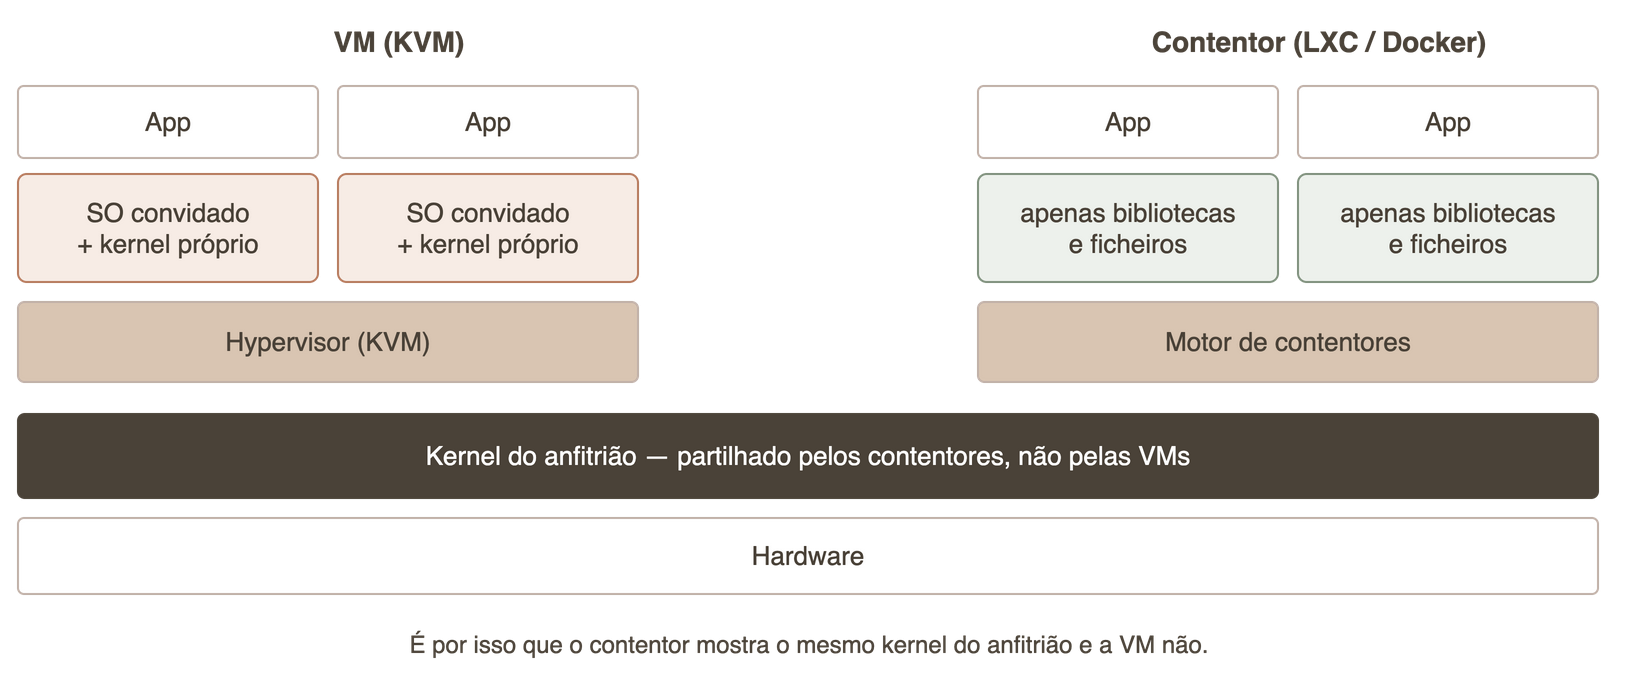
\includegraphics[width=0.97\textwidth,height=0.70\textheight,keepaspectratio]{../Diagramas/a03-vm-vs-contentor.png}
\end{center}
\vfill
\end{frame}


\begin{frame}
\frametitle{Síntese da Aula \textcolor{NudeTaupe}{\small(1/2)}}
\begin{itemize}
    \setlength\itemsep{0.4cm}
    \item A virtualização permite consolidação, isolamento e portabilidade de cargas de trabalho.
    \item Hypervisors tipo 1 (bare-metal) dominam em produção; tipo 2 (hosted) são úteis em desenvolvimento.
    \item Virtualização completa, paravirtualização e suporte de hardware (VT-x/AMD-V) são as três grandes estratégias de virtualização de CPU, todas a lidar com o mesmo problema: instruções sensíveis que o hypervisor tem de apanhar (trap) e emular.
\end{itemize}
\end{frame}

\begin{frame}
\frametitle{Síntese da Aula \textcolor{NudeTaupe}{\small(2/2)}}
\begin{itemize}
    \setlength\itemsep{0.4cm}
    \item Memória, rede e armazenamento são também virtualizados, com mecanismos próprios (EPT, KSM/ballooning, vSwitch, discos qcow2/raw com thin provisioning).
    \item I/O pode ser emulado, passado diretamente à VM (passthrough) ou particionado com SR-IOV, consoante o compromisso entre compatibilidade e desempenho.
    \item Snapshots, clones e templates são as ferramentas operacionais do dia-a-dia; a migração ao vivo (pre-copy, post-copy ou híbrida) permite manutenção sem downtime.
    \item Existe sempre algum overhead; em cenários de desempenho extremo, o bare-metal continua a ser preferível.
    \item KVM (VMs) e LXC (contentores de sistema) coexistem no Proxmox VE, a plataforma usada nesta UC.
\end{itemize}
\end{frame}

\begin{frame}[plain]
  \vspace*{3cm}
  \begin{center}
    \Huge\bfseries\textcolor{TextEspresso}{Obrigada.}\par
    \vspace{0.5cm}
    {\color{NudeTaupe}\rule{2cm}{0.5pt}}\par
    \vspace{0.5cm}
    \Large\textcolor{TextEspresso}{\itshape Questões e comentários}
  \end{center}
\end{frame}

\end{document}
